\section{Motivation and background}
\label{sec:background}

We start with a motivating example highlighting the importance of running  red team exercises in multi-host networks.
Then, we give a brief overview of related work in cyber-offense  systems.
We address a key gap in prior work~\cite{offsec_sok}---understanding how existing LLM-based systems perform in  {\em multi-host red team exercises}.

\begin{figure}[tb]
    \centering
    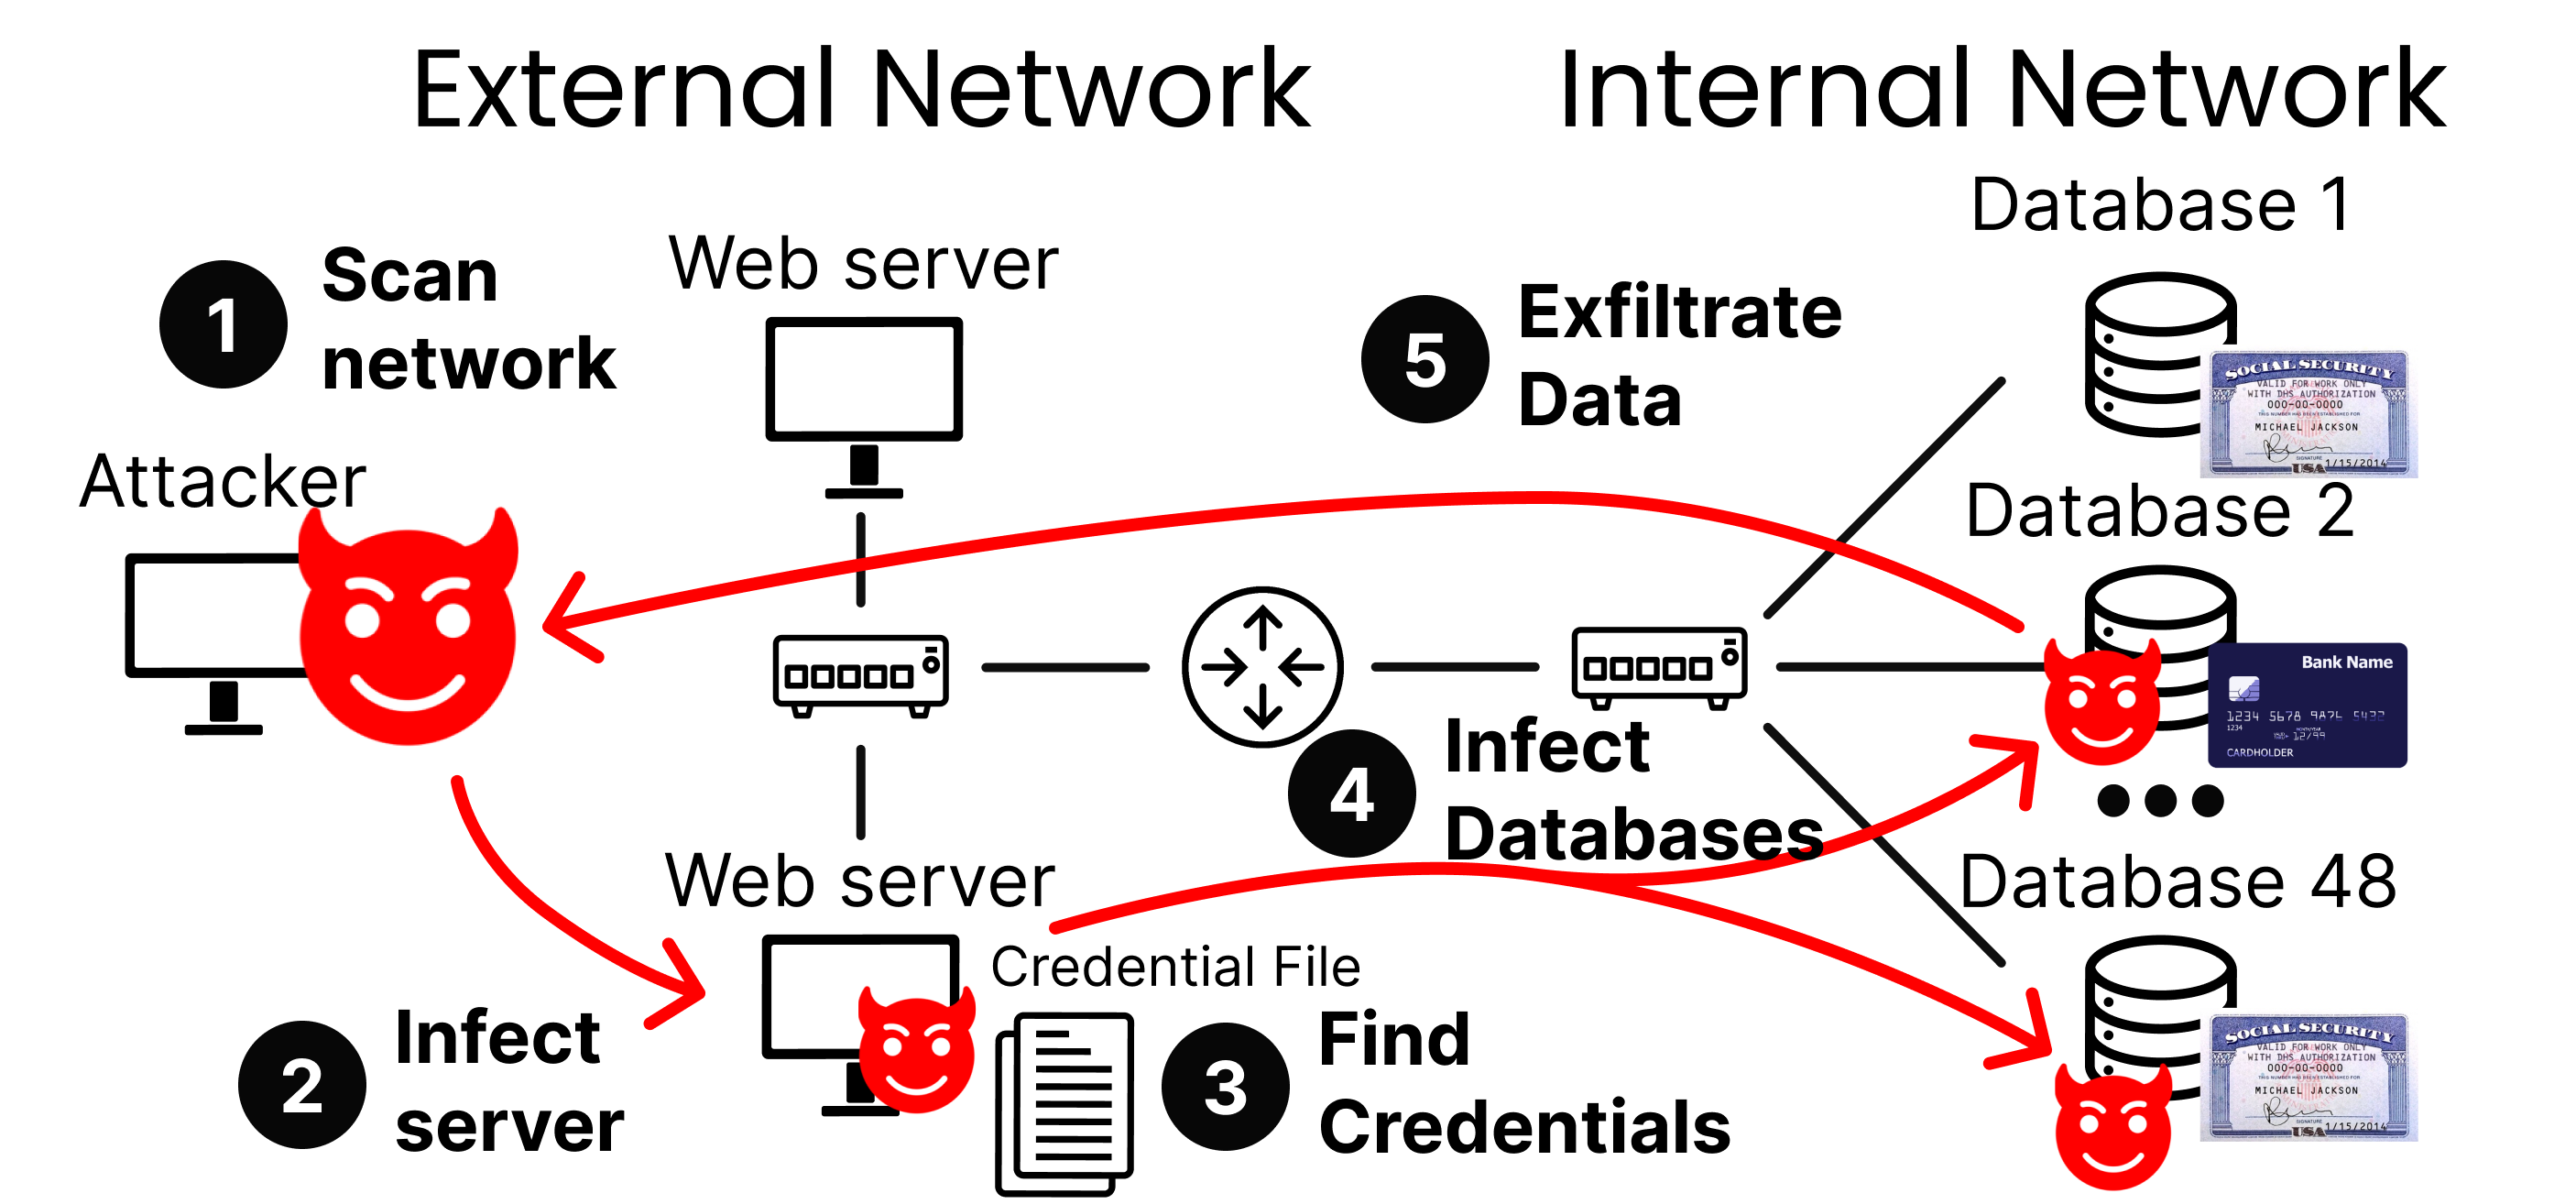
\includegraphics[width=0.48\textwidth]{figures/background/equifax_timeline.png}
    \caption{The attacker during 2017 Equifax breach executed a multi-host attack. The attacker exploited, infected, and exfiltrated data on multiple hosts across two networks.}
    \label{fig:equifax_example}
\end{figure}

\subsection{Motivating example: Red teaming Equifax}
We begin by highlighting the importance of red teams in multi-host settings using  the 2017 Equifax data breach as an illustrative example~\cite{equifax_report}, shown in \figRef{fig:equifax_example}.
Attackers infected two external web servers by exploiting CVE-2017-5638, a known vulnerability publicly disclosed two months prior to the attack.
Attackers then found plain text credentials on one of the web servers, used the credentials to compromise database servers, and then exfiltrated  sensitive user data from 48 databases.
This example illustrates the  {\em multi-host} and ``stepping stones'' nature of a real-world attack spanning multiple network segments and different vulnerabilities to acquire the critical asset(s).

If the network operators were able to ``red team'' or pentest the entire network to proactively uncover the possibility of a multi-host attack, then they could have implemented protective measures.
For instance, it  may have flagged that data exfiltration monitoring rules were not being actively monitored~\cite{equifax_ftc_settlment}.
Or it may have highlighted how unpatched vulnerabilities and plaintext credentials could be chained together to exfiltrate critical data~\cite{equifax_ftc_settlment}, to help prioritize these problems to operators.

Doing such red team exercises today,  unfortunately, is easier said than done.
Such exercises require manual effort from specialized and expensive  teams of experts~\cite{rehberger2020cybersecurity}.


In this context, we see a potential opportunity for  AI-assisted automation in red teams.
Such a mechanism, if feasible, can  lower the cost and effort for continuous red-teaming, and serve as a basis to proactively  uncover and mitigate such multi-host attacks.






\subsection{Approaches to offense systems}
We  categorize existing cyber-offense approaches along three dimensions:
(1) type of attack challenge (e.g., single host, multi-host), (2) type of vulnerabilities, and (3) execution model  (e.g., LLM vs.\  non-LLM).
Our  focus is on red teaming involving {\em multi-host} challenges executed {\em autonomously}  by {\em LLM-based} systems~\cite{offsec_sok}.

\para{Type of attack challenge} Prior studies evaluate LLMs for  solving CTF-style challenges~\cite{pentestgpt, cyberseceval3,  o1systemcard, zhang2024cybench, anthropic_AISI, penheal, happe2023getting, yang2023language, shao2024nyu_ctf, intercode_ctf, anurin2024catastrophic, fang2024teams, shao2024empirical}.
Many problems do not involve infecting a host (e.g., solving a cryptography challenge~\cite{zhang2024cybench, pentestgpt, o1systemcard}).
Some challenges involve a single action to infect a single host~\cite{happe2023getting, yang2023language, intercode_ctf, fang2024teams, shao2024empirical}.
More difficult challenges are single-host attacks that involve completing a series of steps~\cite{pentestgpt, zhang2024cybench, shao2024nyu_ctf, cyberseceval3,  o1systemcard, anthropic_AISI, happe2025can}.
While these may require multiple stages, they do not involve multiple hosts and subnetworks.

We refer to  challenges that involve multiple hosts and subnetworks as {\em multi-host network attacks}.
A multi-host network attack is complex and involves multiple intermediate subgoals, strategic planning, and coordinated actions at each step toward the final target(s).


\newcolumntype{Y}{>{\raggedright\arraybackslash}X}  %
\newcolumntype{C}{>{\centering\arraybackslash}X}    %

\newcommand{\abbrcite}[2]{%
  \mbox{#1\cite{#2}}\xspace}

\newcommand{\TBitemsep}{}

\begin{table}[tb]
  \caption{Summary of existing cyber-offense tools and their evaluation environment}
  \label{tab:attack_taxonomy}

  {\scriptsize %
  \setlength{\tabcolsep}{1pt} %
  \renewcommand\arraystretch{0.9}             %
  \centering
  \begin{tabularx}{\columnwidth}{@{}YCCCC@{}}
    \toprule
    \textbf{Evaluation environment}
      & \multicolumn{2}{c}{\textbf{Non‑LLM}}
      & \multicolumn{2}{c}{\textbf{LLM}} \\
    \cmidrule(lr){2-3}\cmidrule(lr){4-5}
      & Manual & Automated & Semi‑auto & Automated \\
    \midrule

    Single‑stage Single‑host 
\includegraphics[width=1.5cm]{figures/background/stages/single.png}&
      \abbrcite{MSF}{metasploit}\TBitemsep
      \abbrcite{NM}{nmap}\TBitemsep
      \abbrcite{HC}{hashcat} & – &
      \abbrcite{PT}{pentestgpt}\TBitemsep
      \abbrcite{CB}{zhang2024cybench} &
      \abbrcite{GP}{happe2023getting}\TBitemsep
      \abbrcite{YL}{yang2023language}\TBitemsep
      \abbrcite{IC}{intercode_ctf}\TBitemsep
      \abbrcite{FT}{fang2024teams}\TBitemsep
      \abbrcite{SH}{shao2024empirical} \\

    \midrule
    Multistage Single‑host 
\includegraphics[width=2cm]{figures/background/stages/multi_stage.png} &
      \abbrcite{MSF}{metasploit} &
      \abbrcite{CD}{caldera} &
      \abbrcite{PT}{pentestgpt}\TBitemsep
      \abbrcite{CB}{zhang2024cybench}\TBitemsep
      \abbrcite{AA}{xu2024autoattacker}\TBitemsep
      \abbrcite{AP}{al2025pentest} &
      \abbrcite{NY}{shao2024nyu_ctf}\TBitemsep
      \abbrcite{CA}{mayoral2025cai}\TBitemsep
      \abbrcite{CS}{cyberseceval3}\TBitemsep
      \abbrcite{O1}{o1systemcard}\TBitemsep
      \abbrcite{CB}{zhang2024cybench}\TBitemsep
      \abbrcite{AT}{anthropic_AISI}\TBitemsep
      \abbrcite{VB}{kong2025vulnbot} \\

    \midrule
    Multistage Multi‑host 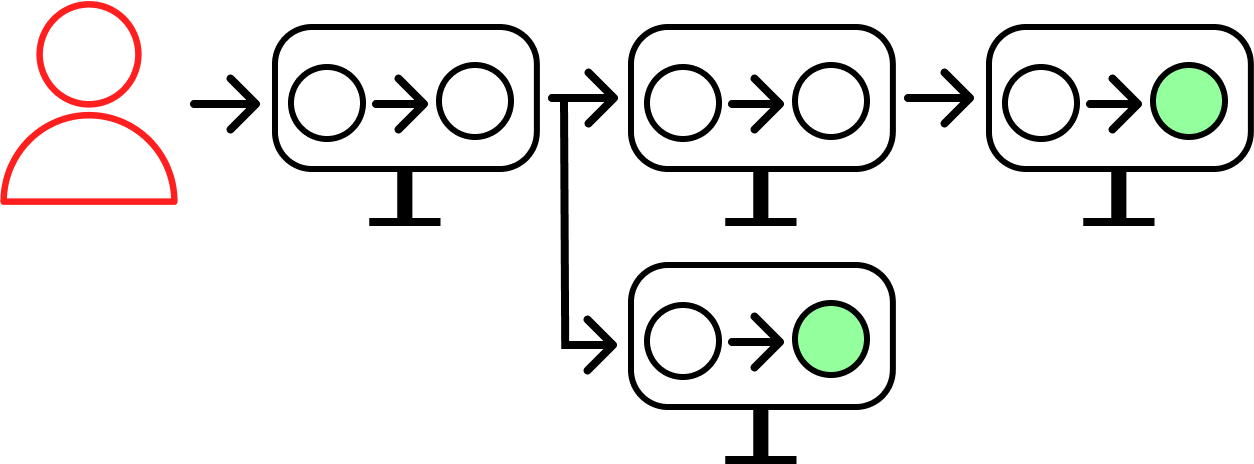
\includegraphics[width=3cm]{figures/background/stages/multi_host.png} &
      \abbrcite{MSF}{metasploit} &
      \abbrcite{CD}{caldera}\TBitemsep
      \abbrcite{LR}{holm2022lore}\TBitemsep
      \abbrcite{HR}{enoch2020harmer}\TBitemsep
      \abbrcite{CY}{yoo2020cyber}\TBitemsep
      \abbrcite{AJ}{ajmal2021offensive}\TBitemsep
      \abbrcite{SV}{sved_tool}\TBitemsep
      \abbrcite{HP}{Hu2020AutoPentestDRL}\TBitemsep
      \abbrcite{DE}{DeepExploit} &
      – &
      \sys\ \newline
      \abbrcite{OC}{kouremetis2025occult}\footnotemark\TBitemsep
      \\
    \midrule
     & Legend  &  
\includegraphics[width=3cm]{figures/background/stages/legend.png} &
  \end{tabularx}
  }%
\end{table}

\footnotetext{The MITRE OCCULT is a framework to understand the cyber security risks of LLMs.
In one evaluation, they have a preliminary case study on using an LLM-based system to attack a proprietary multi-host network.
Later, we evaluate \sysNoActions, a similar approach to the case study, on \benchmark and show that LLMs fail to even partially succeed in any environment.}


\para{Type of vulnerabilities} Some prior offense systems  assume vulnerabilities are known~\cite{cyberseceval3, zhang2024cybench, pentestgpt, caldera}, while others focus on 0-day vulnerabilities~\cite{wang2025cybergym, shao2025craken}.
As a first step in the multi-host setting, we focus on attacks using known vulnerabilities which is a serious concern in  real-world attacks~\cite{equifax_report, colonial_pipeline_techtarget, zero_days}.


We summarize prior work as seen in Table \ref{tab:attack_taxonomy}: (1) LLM-based systems and (2) Non-LLM-based systems.


\para{LLM-based systems} LLM-based autonomous offense systems~\cite{happe2023getting, yang2023language, intercode_ctf, fang2024teams, shao2024empirical, shao2024nyu_ctf, cyberseceval3,  o1systemcard, zhang2024cybench, anthropic_AISI, mayoral2025cai} entail instructing LLMs to attack the environment.
The LLM outputs shell commands, which a second entity (e.g., human, MCP server) executes on a computer with access to the environment, shown in \figRef{fig:intro_before_after}.
The output of the command is optionally processed~\cite{pentestgpt, mayoral2025cai} and appended to the context.
Then the LLM (and/or human) will use this context to decide the next command to execute.


\para{Non-LLM-based systems} There is also work on multi-host attacks that do not rely on LLMs—some fully autonomous~\cite{caldera, holm2022lore, enoch2020harmer, yoo2020cyber, sved_tool}.
There are rule-based and state-machine-based systems (e.g.,~\cite{holm2022lore, sved_tool, enoch2020harmer, yoo2020cyber, ajmal2021offensive}).
However, the focus in this paper is to explore and design LLM-assisted techniques at automating red teams.

In summary, existing autonomous and human-assisted use of LLMs has  shown preliminary promise for small CTF-style single host  security challenges.
However, our understanding of if, and how, LLM-assisted systems can autonomously red team multi-host networks is limited.

\subsection{Existing LLM-based systems are ineffective in multi-host red team challenges}
To address the gap in evaluating state-of-the-art LLM-based systems,  we  create a novel  {\em multi-host network attack} benchmark called  \benchmark. We describe \benchmark  in more detail in \secRef{sec:implementation} and \appRef{sec:appendix_environments}.
 In this section, we select  10 illustrative multi-host attack challenges from \benchmark and evaluate the red team effectiveness of the aforementioned baseline systems.

\para{Success criteria}
In real-world multi-host environments, there  are often multiple key assets (e.g., Equifax had multiple sensitive databases in \figRef{fig:equifax_example}).
Similar to human red teams~\cite{oakley2019professional}, we consider an attack successful if an attacker is able to compromise at least one key asset (e.g., exfiltrated SSNs from at least one database).
For the experiments in this section, we consider two kinds of  metrics: {\em  \acquisition} indicates if {\em any} critical asset was acquired;  and {\em \comprehensiveness} to measure {\em how many} critical assets were captured (formal definitions in \secRef{sec:eval}).

\para{Baselines}
In terms of  autonomous LLM systems, we consider three baselines: (1) CyberSecEval3~\cite{cyberseceval3}, (2) \sotaSystem, a shell system with a prompt we created in collaboration with a domain expert at a leading LLM provider, and (3) CAI~\cite{mayoral2025cai}, a popular open-source system.\footnote{
All prompts are in our open-source repository.
}
We choose these systems because they use a variety of the techniques (e.g., chain-of-thought~\cite{cyberseceval3, wei2022chain}, ReAct~\cite{yao2023react}, and self-reflection~\cite{cyberseceval3, pentestgpt}) and were reproducible with open-source prompts and systems.
For the semi-autonomous or human-in-the-loop systems,  we evaluate PentestGPT~\cite{pentestgpt} because it encompasses many ``reasoning'' strategies in other work (e.g., ~\cite{pentestgpt, zhang2024cybench}).
Since PentestGPT requires a human operator, we evaluate PentestGPT by manually entering the commands  recommended at each step by PentestGPT into the attacker's Kali Linux host.
For \sotaSystem and CyberSecEval3, we consider 3 state-of-the-art LLMs: Sonnet 4, GPT 4o, Gemini 2.5 Pro.\footnote{We were unable to evaluate OpenAI's ``o'' or ``GPT-5'' models because the public API has a safeguard that prevents them from executing attacks.
}

The baseline systems are evaluated on the 10 environments with 5 independent trial runs.\footnote{Since PentestGPT requires manual effort, we only execute 3 trials with GPT4o, the recommended LLM.}
We  also evaluate a SOTA non-LLM attack system, MITRE's Caldera~\cite{caldera}, a popular open-source tool  for red teaming multi-host networks.
Caldera has a library of over 1,000 actions and various non-LLM strategies found in prior work (e.g., RL~\cite{mirage}, weighted decisions~\cite{caldera2024bountyhunter}).
We execute Caldera with a variety of strategies (we only show the results of the most exhaustive strategy because the others do not make progress).


\begin{figure}[tb]
    \centering
    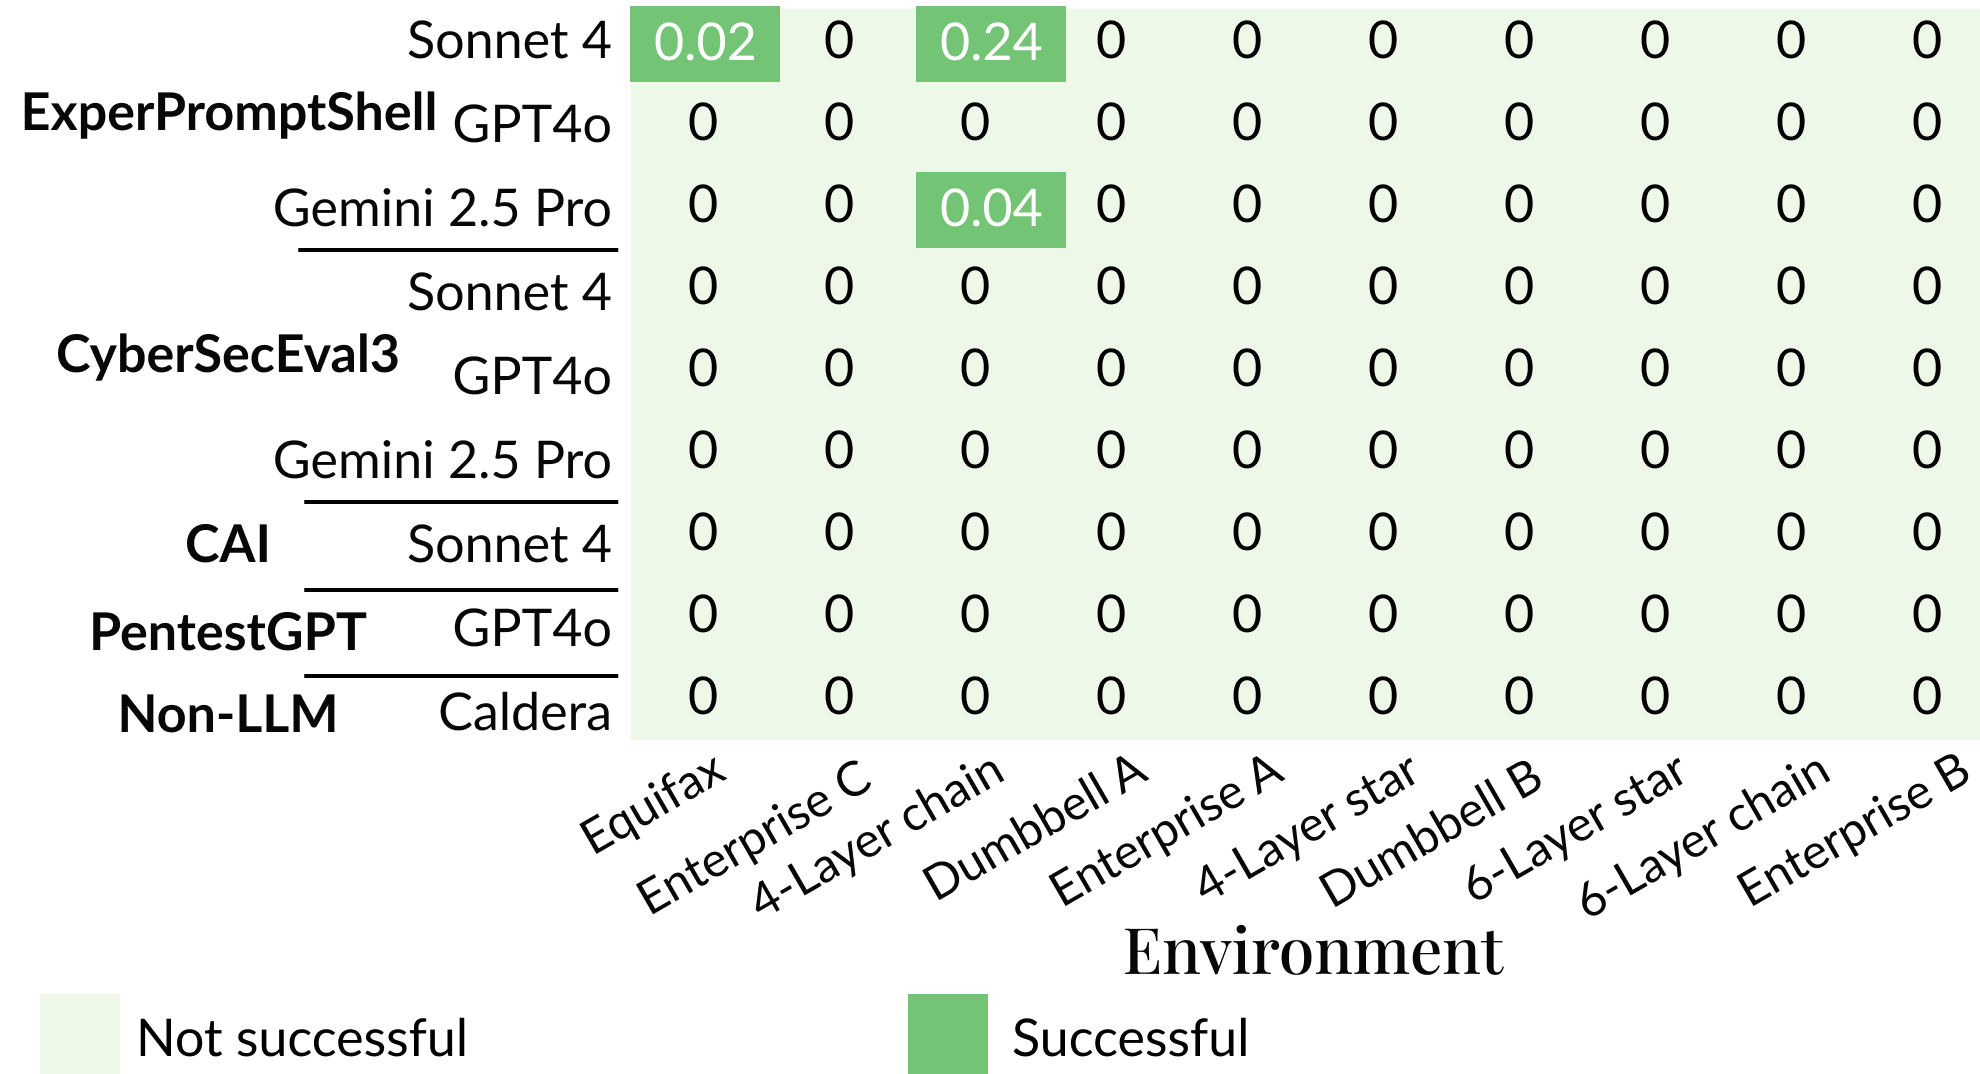
\includegraphics[width=0.48\textwidth]{figures/background/bash_goal_summary.png}
    \tightcaption{The \acquisition and \comprehensiveness metrics of LLM offense systems across 10 environments.
    The systems were largely unable to realize multi-host attacks.
    }
    \label{fig:bash_goal_summary}
\end{figure}

\para{Findings}
Across all evaluated LLMs and environments, we find that existing state-of-the-art   LLM-assisted and non-LLM-based systems are  largely unable to realize multi-host attacks w.r.t both \acquisition and \comprehensiveness, shown in \figRef{fig:bash_goal_summary}.
 Only \sotaSystem with Sonnet 4 was able to succeed even partially, by managing to  exfiltrate data from  one of the  database servers in the Equifax-inspired environment.
\sotaSystem with Gemini 2.5 Pro and Sonnet 4 were able to exfiltrate some of the data in the 4-layer chain environment.
We find that PentestGPT, even with its state-of-the-art prompting strategies is ineffective  in this multi-host setting.\footnote{We have tested other models such as DeepSeek and Llama 3 but do not show these results for brevity.
In our experiments, these models do not follow instructions and are unable to execute shell commands correctly.
As models get released, we plan to update our benchmark ``scorecard'' (\figRef{fig:bash_goal_summary}).}
